\documentclass{article}
\usepackage[margin=1in]{geometry} %1 in margins
\usepackage{graphicx} %For including graphics
\usepackage[labelfont=bf]{caption} %Make float labels bold
\usepackage{subcaption}
\usepackage{amsmath}    
\usepackage{listings}% http://ctan.org/pkg/listings
\lstset{
  basicstyle=\ttfamily,
  mathescape
}
\usepackage{hyperref}
\renewcommand{\floatpagefraction}{0.95}
\renewcommand{\topfraction}{0.95}
\renewcommand{\textfraction}{0.05}
\usepackage{url}

% Define a ``Program'' float for code
\usepackage{verbatim} %Allow verbatim input for code
\usepackage{float} %Defining the Program environment
\floatstyle{boxed}
\newfloat{program}{htbp}{pgm}
\floatname{program}{Program}



\begin{document}

\begin{center}
{\Large {\bf Solution to Homework \#2---MTH 522} }

Mehmet Duman
\end{center}

{\bf Problem 1} (Chapter 3 Exercises 8):This question involves the use of simple linear regression on the Auto data set.

\begin{itemize}
\item[(a)]  Use the lm() function to perform a simple linear regression with mpg as the response and horsepower as the predictor. Use the summary() function to print the results. Comment on the output.

\item[(i)] Is there a relationship between the predictor and the response ?


\begin{program}
	\begin{verbatim}
> setwd('/Users/ekinezgi/Documents/UmassD/MTH_522_Istatistical_Learning2016F/Data/')
> Auto = read.csv("Auto.csv" , header=T, na.strings="?")
> Auto=na.omit(Auto)
> fit <- lm(mpg ~ horsepower, data = Auto)
> summary(fit)

Call:
lm(formula = mpg ~ horsepower, data = Auto)

Residuals:
Min                1Q            Median                3Q               Max 
-13.5710402197074  -3.2591510181224  -0.3435429524515   2.7630327970151  16.9240466468170 

Coefficients:
Estimate         Std. Error   t value   Pr(>|t|)    
(Intercept) 39.935861021170489  0.717498655554526  55.65984 < 2.22e-16 ***
horsepower  -0.157844733353654  0.006445500517685 -24.48914 < 2.22e-16 ***
---
Signif. codes:  0 ‘***’ 0.001 ‘**’ 0.01 ‘*’ 0.05 ‘.’ 0.1 ‘ ’ 1

Residual standard error: 4.905756919546 on 390 degrees of freedom
(5 observations deleted due to missingness)
Multiple R-squared:  0.6059482578894,	Adjusted R-squared:  0.6049378688071 
F-statistic: 599.7177409016 on 1 and 390 DF,  p-value: < 2.2204460493e-16
\end{verbatim}
\end{program}


$H_0 : B\_mpg = B\_horsepower = 0$
\newline
In Section 3.2.2, it showed that the F-statistic can be used to determine whether or not we should reject this null hypothesis. In this case the p-value ( $<$ 2.2e-16)  corresponding to the F-statistic ( 599.7 on 1 and 390 DF)  is very low, indicating clear evidence of a relationship between mpg and horsepower.



\item[(ii)] How strong is the relationship between the predictor and the response?

\begin{program}
	\begin{verbatim}
	> mean(Auto[["mpg"]])	               ##  mean of mpg
	[1] 23.44591836734694
	
	> summary(fit)$sigma                 ##  Residual standard error
	[1] 4.90575691954594
	
	> 4.90575691954594 / 23.44591836734694
	[1] 0.2092371406691483
	\end{verbatim}
\end{program}

The RSE estimates the standard deviation of the response from the population regression line (3.4 ,Page 102).
The Residual standard error of fit was 4.90575691954594 which indicates percentage error of 20.9237\% 
\newline
The $R^2$ statistic records the percentage of variability in the response that is explained by the predictors (3.4 ,Page 102).
$R^2$ is equal to 0.6059482578894, almost 60.59482578894\% of the variability in “mpg” can be explained using “horsepower”.


\item[(iii)]  Is the relationship between the predictor and the response positive or negative?

The coeficient of “horsepower” is negative so, the relationship between horsepower and mpg is also negative. More horsepower means less mpg fuel efficiency the car will have.


\item[(iv)]  What is the predicted mpg associated with a horsepower of 98? 

\begin{program}
	\begin{verbatim}
> predict(fit, data.frame(horsepower = 98), interval = "confidence")
fit                         lwr                  upr
1 24.46707715251241   23.9730789607039   24.96107534432091


> predict(fit, data.frame(horsepower = 98), interval = "prediction")
fit                        lwr                upr
1 24.46707715251241   14.8093960709667   34.12475823405811

\end{verbatim}
\end{program}

\newpage
\item[(b)]  Plot the response and the predictor. Use the abline() function to display the least squares regression line.

\begin{program}
	\begin{verbatim}

> attach(Auto)
> plot(horsepower, mpg)
> abline(fit ,col="red")
> dev.copy(png,"MTH522_hw2_p1b.png",width=8,height=6,units="in",res=200)
> dev.off()

	\end{verbatim}
\caption{The R code used to generate Figure.\ \ref{fig:MTH522_hw2_p1b}.}
\end{program}


\begin{figure}[htb]
	\begin{center}
		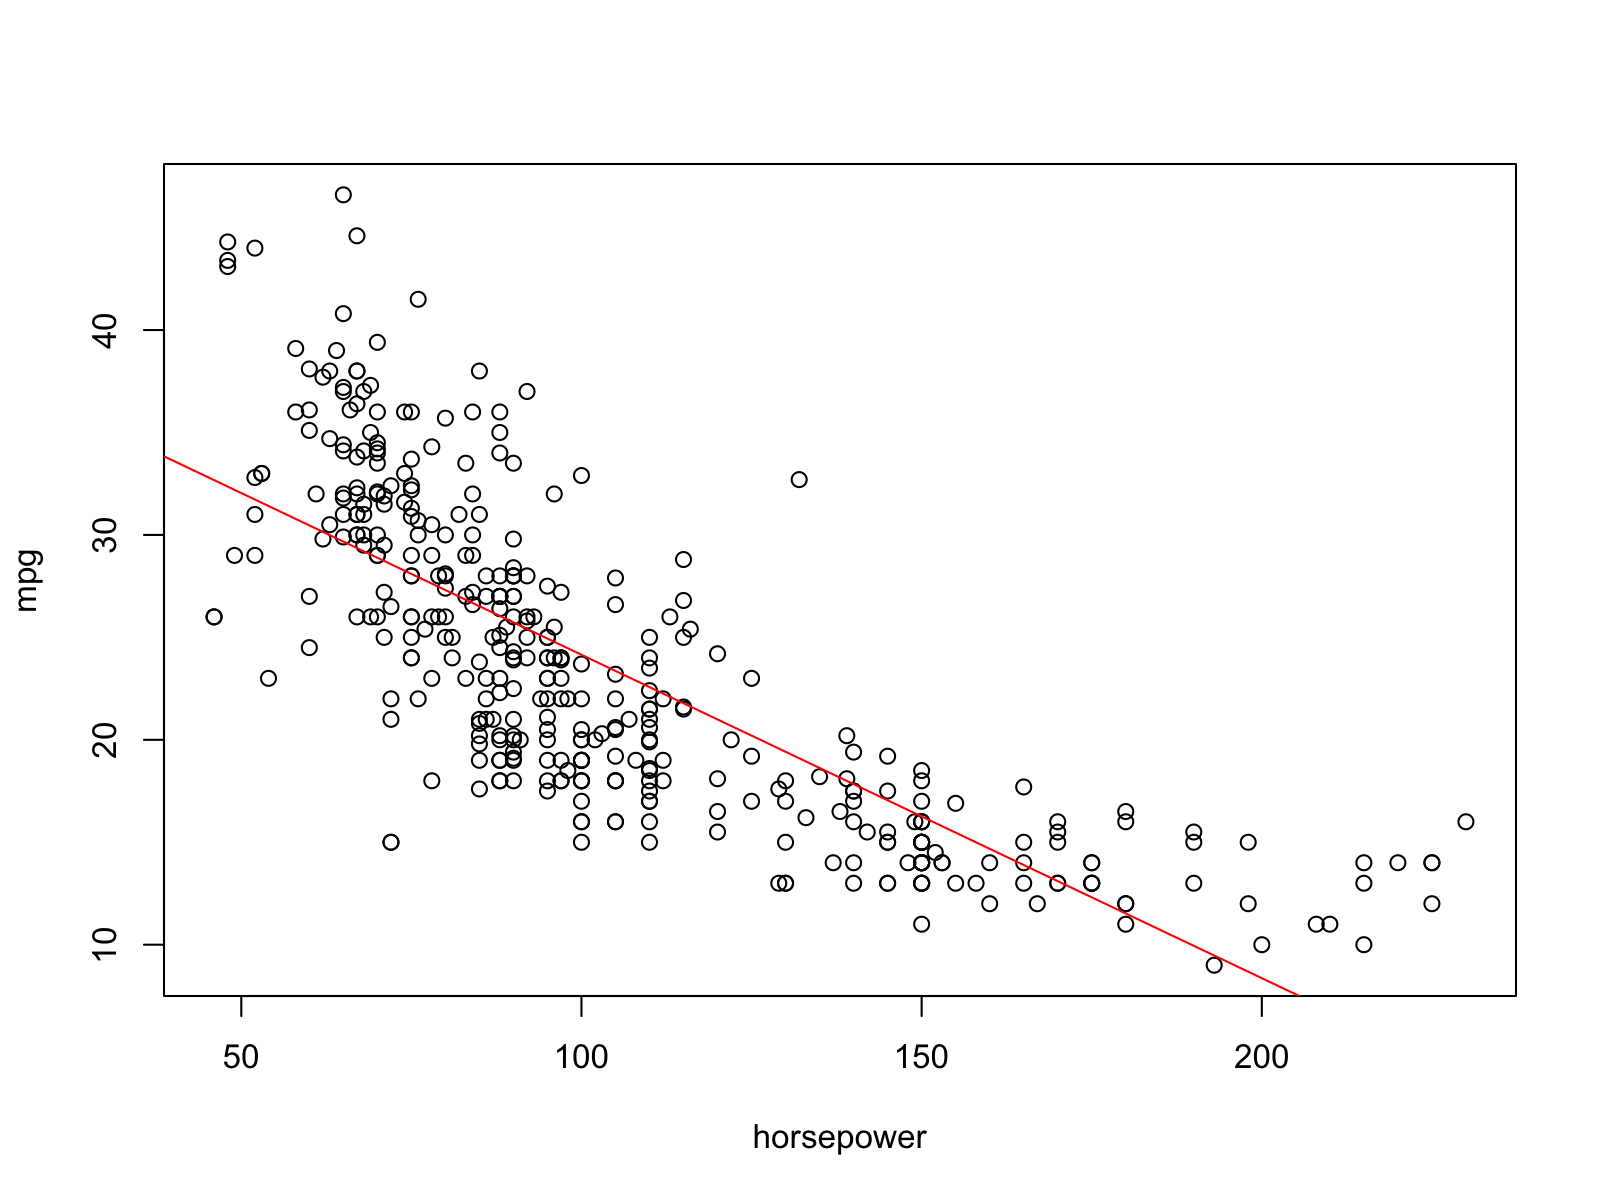
\includegraphics[width=0.8\textwidth]{MTH522_hw2_p1b.png}
	\end{center}
	\caption{.}
	\label{fig:MTH522_hw2_p1b}
\end{figure}








\newpage
\item[(c)]  Use the plot() function to produce diagnostic plots of the least squares regression fit.

\begin{program}
	\begin{verbatim}
	
> par(mfrow = c(2, 2))
> plot(fit)
> dev.copy(png,"MTH522_hw2_p1c.png",width=8,height=6,units="in",res=200)
> dev.off()
	
	\end{verbatim}
	\caption{The R code used to generate Figure.\ \ref{fig:MTH522_hw2_p1c}.}
\end{program}


\begin{figure}[htb]
	\begin{center}
		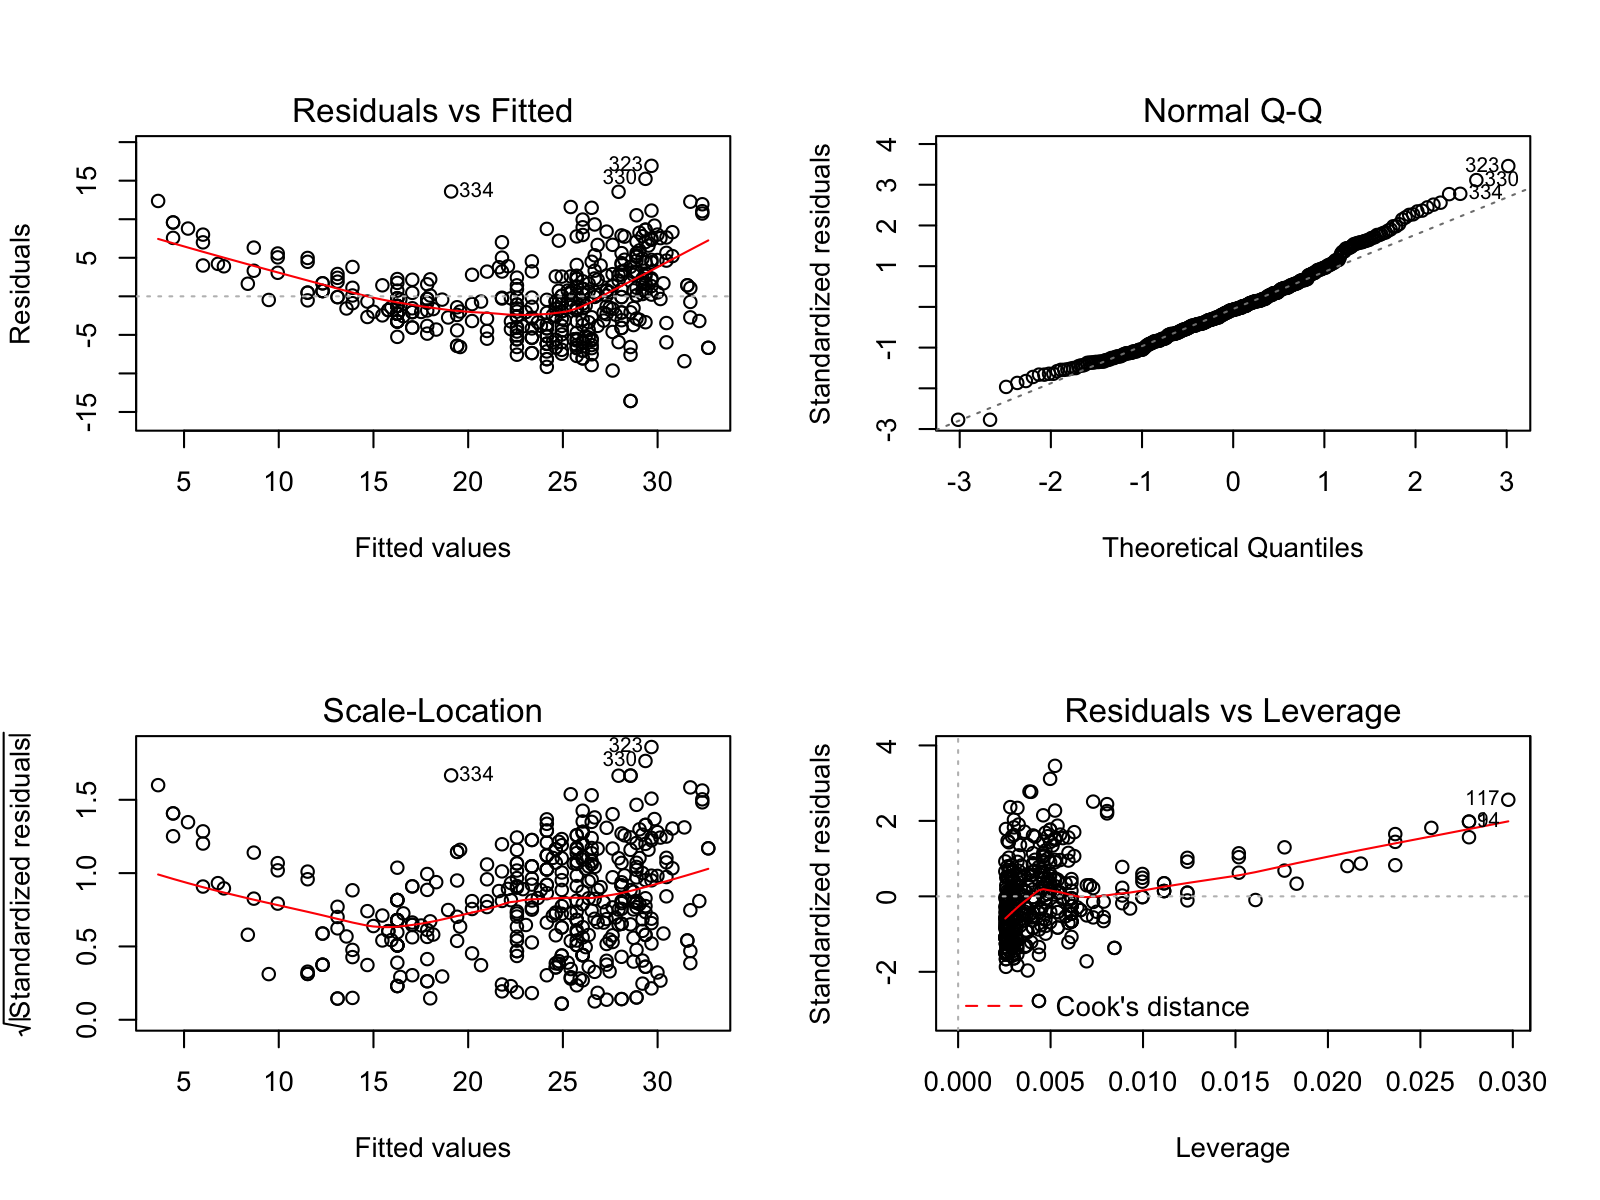
\includegraphics[width=0.8\textwidth]{MTH522_hw2_p1c.png}
	\end{center}
	\caption{.}
	\label{fig:MTH522_hw2_p1c}
\end{figure}

Residuals vs Fitted : The red line is a smooth fit to the residuals, a strong pattern in the residuals indicates non-linearity in the data. (same as Figure 3.9 Page:93)
 




\newpage
{\bf Problem 2} (Chapter 3 Exercises 9):This question involves the use of multiple linear regression on the Auto data set.
\item[(a)] Produce a scatterplot matrix which includes all of the variables in the data set

\begin{program}
\begin{verbatim}

> par(mfrow = c(9, 9))
> pairs(Auto)	
> dev.copy(png,"MTH522_hw2_p2a.png",width=8,height=6,units="in",res=200)
> dev.off()
	
\end{verbatim}
\caption{The R code used to generate Figure.\ \ref{fig:MTH522_hw2_p2a}.}
\end{program}


\begin{figure}[htb]
	\begin{center}
		
\includegraphics[width=0.8\textwidth]{MTH522_hw2_p2a.png}
	\end{center}
	\caption{.}
	\label{fig:MTH522_hw2_p2a}
\end{figure}


\newpage

\item[(b)] Compute the matrix of correlations between the variables using the function cor(). You will need to exclude the name variable, which is qualitative.

\begin{program}
\begin{verbatim}
> options(digits=4)
> cor(subset(Auto, select=-name))	
\end{verbatim}
\caption{The R code used to generate outputFigure.\ \ref{fig:MTH522_hw2_p2b}.}
\end{program}


\begin{figure}[htb]
	\begin{center}
		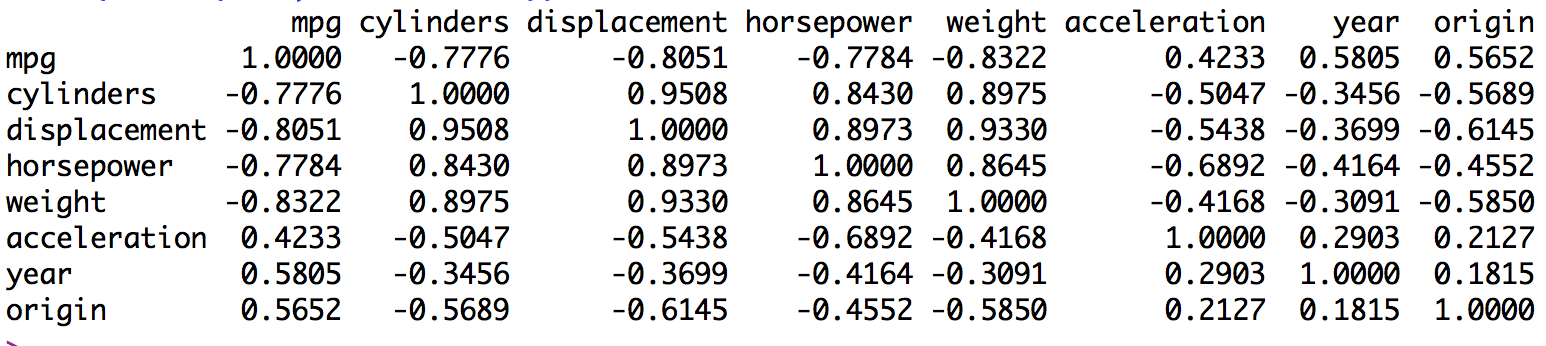
\includegraphics[width=0.8\textwidth]{MTH522_hw2_p2b.png}
	\end{center}
	\caption{.}
	\label{fig:MTH522_hw2_p2b}
\end{figure}

\item[(c)] Use the lm() function to perform a multiple linear regression with mpg as the response and all other variables except name as the predictors. Use the summary() function to print the results. Comment on the output. For instance:


\newpage

\item[(i)] Is there a relationship between the predictors and the response?

\begin{program}
\begin{verbatim}
> options(digits=16)
> fit2 <- lm(mpg ~ . - name, data = Auto)
> summary(fit2)

Call:
lm(formula = mpg ~ . - name, data = Auto)

Residuals:
Min               1Q           Median               3Q              Max 
-9.5902611207376 -2.1565164908716 -0.1169410096327  1.8689660525158 13.0604272507154 

Coefficients:
Estimate          Std. Error  t value   Pr(>|t|)    
(Intercept)  -1.721843462202e+01  4.644294149424e+00 -3.70744 0.00024018 ***
cylinders    -4.933763188585e-01  3.232823146374e-01 -1.52615 0.12779647    
displacement  1.989564374202e-02  7.515079164719e-03  2.64743 0.00844465 ** 
horsepower   -1.695114422750e-02  1.378689141407e-02 -1.22951 0.21963282    
weight       -6.474043397441e-03  6.520477605638e-04 -9.92879 < 2.22e-16 ***
acceleration  8.057583832486e-02  9.884495665657e-02  0.81517 0.41547802    
year          7.507726779503e-01  5.097312225270e-02 14.72880 < 2.22e-16 ***
origin        1.426140495423e+00  2.781360923898e-01  5.12749 4.6657e-07 ***
---
Signif. codes:  0 ‘***’ 0.001 ‘**’ 0.01 ‘*’ 0.05 ‘.’ 0.1 ‘ ’ 1

Residual standard error: 3.327682396407 on 384 degrees of freedom
Multiple R-squared:  0.8214780764811,	Adjusted R-squared:  0.8182237705836 
F-statistic: 252.4280452913 on 7 and 384 DF,  p-value: < 2.2204460493e-16
\end{verbatim}
	\caption{.}
\end{program}


All the regression coefficients are zero.
Yes, In this case the p-value ( $<$ 2.2204460493e-16)  corresponding to the F-statistic ( 252.4280452913 on 7 and 384 DF)  is very low, indicating clear evidence of a relationship between mpg and the other predictors except name.


\item[(ii)] Which predictors appear to have a statistically significant relationship to the response?
\newline

When we check the p-values associated with each predictor's t-statistic.

\begin{program}
\begin{verbatim}
weight         -9.93   2.00E-16
year           14.73   2.00E-16
origin          5.13	  4.70E-07
displacement    2.65   0.00844
cylinders      -1.53   0.1278
horsepower     -1.23   0.21963
acceleration    0.82   0.41548
\end{verbatim}
\end{program}
It shows that weight, year, origin and displacement have a statistically significant relationship, but
cylinders, horsepower and acceleration do not have a statistically significant relationship to the response.


\item[(iii)] What does the coefficient for the year variable suggest?

The coefficient for the year : 7.507726779503e-01 = 0.7507726779503
It suggest that 1 of "year" increase will effect 0.7507726779503 increase in "mpg" . 
Every year cars will be 0.7508 mpg/yer more fuel efficent 





\item[(d)] Use the plot() function to produce diagnostic plots of the linear regression fit. Comment on any problems you see with the fit. Do the residual plots suggest any unusually large outliers? Does the leverage plot identify any observations with unusually high leverage?



\begin{program}
\begin{verbatim}
	
> par(mfrow=c(2,2))
> plot(fit2)
> dev.copy(png,"MTH522_hw2_p2d.png",width=8,height=6,units="in",res=200)
> dev.off()
\end{verbatim}
\caption{The R code used to generate Figure.\ \ref{fig:MTH522_hw2_p2d}.}
\end{program}


\begin{figure}[htb]
	\begin{center}
		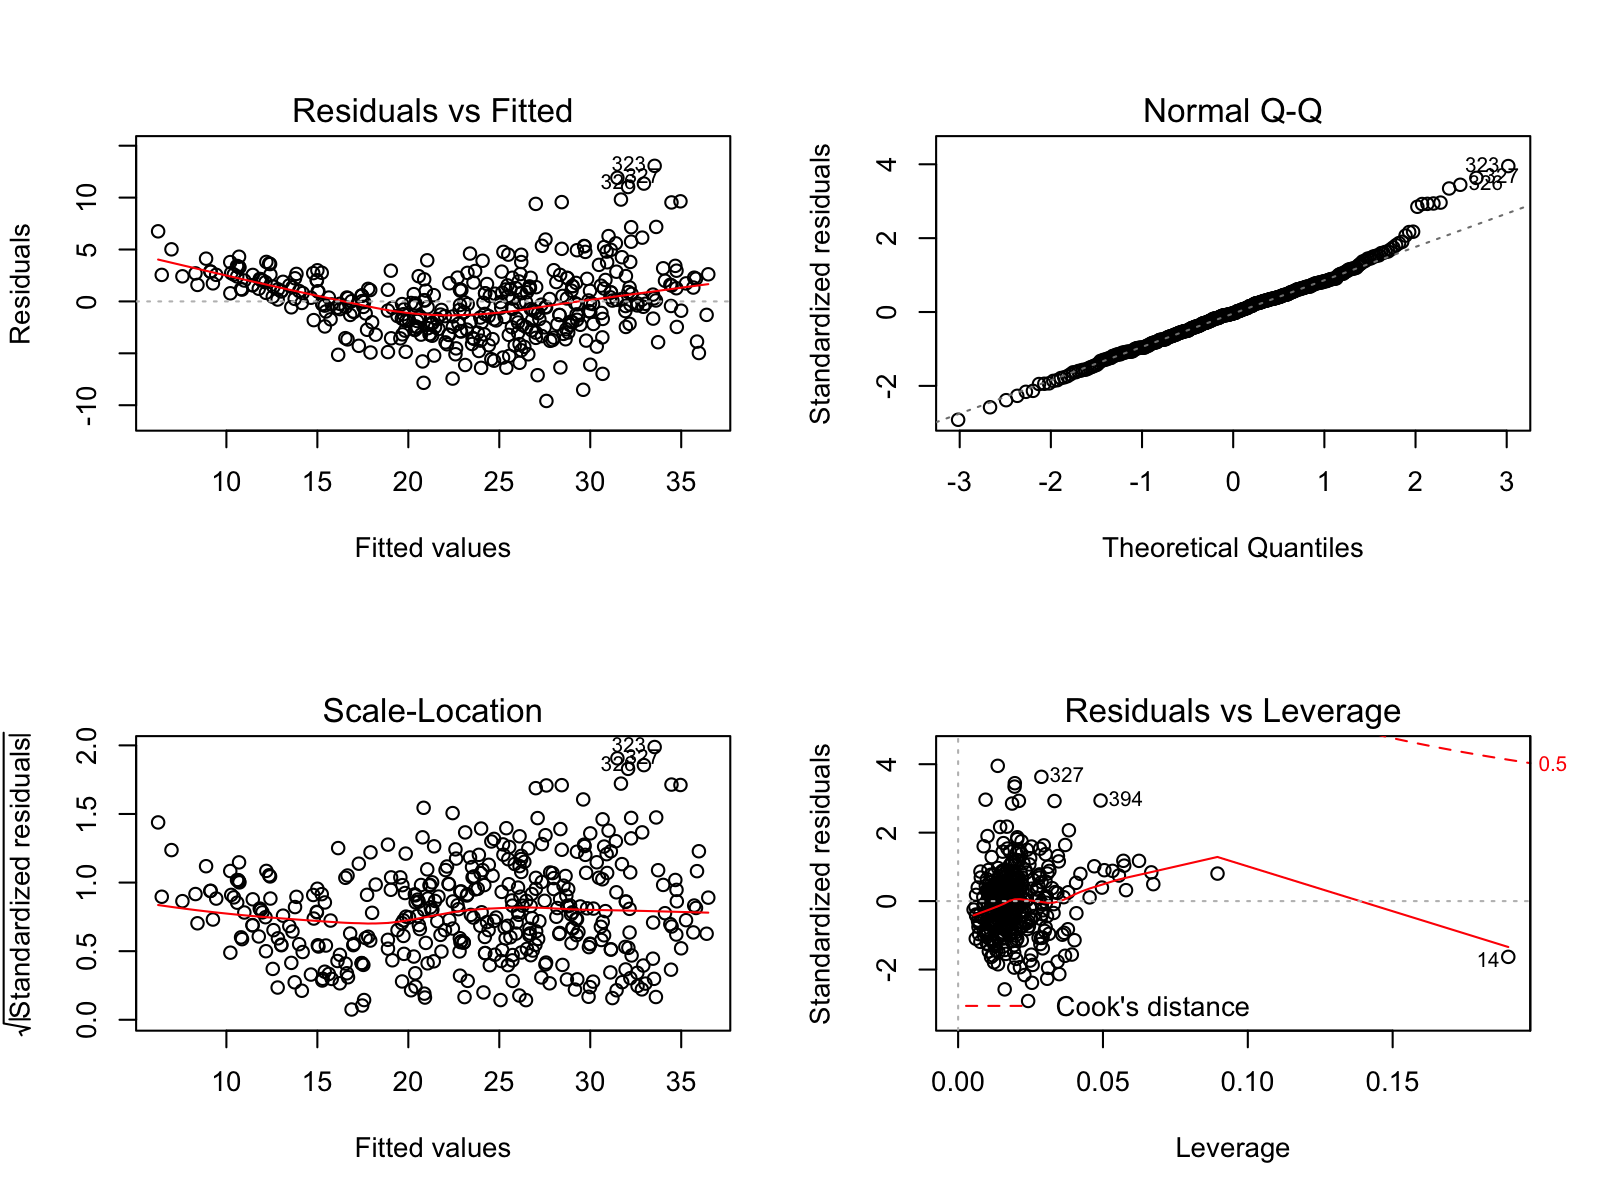
\includegraphics[width=0.8\textwidth]{MTH522_hw2_p2d.png}
	\end{center}
	\caption{.}
	\label{fig:MTH522_hw2_p2d}
\end{figure}

Residuals vs Fitted : The red line is a smooth fit to the residuals, a strong pattern in the residuals indicates non-linearity in the data. (same as Figure 3.9 Page:93)
\\Residuals vs Leverage : Point 14 is high leverage point and some outliers point out of [-2,2].



\newpage

\item[(e)] Use the * and : symbols to fit linear regression models with interaction effects. Do any interactions appear to be statistically significant?



Corelation matrix from probllem 2b:  I took two highest correlated pairs:
\\cylinders      * displacement..: 0.9508
\\displacement *  weight.........:  0.9330 

\begin{program}
	\begin{verbatim}
	
	> fit3 <- lm(mpg ~ cylinders * displacement+displacement * weight, data = Auto[, 1:8])
	> summary(fit3)
	
	Call:
	lm(formula = mpg ~ cylinders * displacement + displacement * 
	weight, data = Auto[, 1:8])
	
	Residuals:
	Min                1Q            Median                3Q               Max 
	-13.2934254366870  -2.5184257440537  -0.3476219470012   1.8398911647246  17.7723233627659 
	
	Coefficients:
	                                  Estimate          Std. Error t value   Pr(>|t|)    
	(Intercept)             5.262340982860e+01  2.237444963766e+00 23.51942 < 2.22e-16 ***
	cylinders               7.606405125175e-01  7.669492027411e-01  0.99177    0.32193    
	displacement           -7.351277340896e-02  1.669463994455e-02 -4.40338 1.3818e-05 ***
	weight                 -9.888166989519e-03  1.329427603832e-03 -7.43791 6.6869e-13 ***
	cylinders:displacement -2.986050976421e-03  3.425719705600e-03 -0.87166    0.38394    
	displacement:weight     2.127741189094e-05  5.001712407694e-06  4.25403 2.6377e-05 ***
	---
	Signif. codes:  0 ‘***’ 0.001 ‘**’ 0.01 ‘*’ 0.05 ‘.’ 0.1 ‘ ’ 1
	
	Residual standard error: 4.102715004849 on 386 degrees of freedom
	Multiple R-squared:  0.7272237222366,	Adjusted R-squared:  0.723690350763 
	F-statistic: 205.8158129328 on 5 and 386 DF,  p-value: < 2.2204460493e-16
	
	\end{verbatim}
\end{program}

The "p-values" shows that interaction between displacement and weight is statistically significant, but
cylinders and displacement is not.



\newpage


\item[(f)] Try a few different transformations of the variables, such as $ log(X), \sqrt{X}, X^2 $. Comment on your findings.


I will do different transformations for "weight" and "horsepower"

\begin{program}
	\begin{verbatim}
	> par(mfrow = c(2, 3))
	> plot(log(Auto$weight), Auto$mpg)
	> plot(sqrt(Auto$weight), Auto$mpg)
	> plot((Auto$weight)^2, Auto$mpg)

	> plot(log(Auto$horsepower), Auto$mpg)
	> plot(sqrt(Auto$horsepower), Auto$mpg)
	> plot((Auto$horsepower)^2, Auto$mpg)
	
	> dev.copy(png,"MTH522_hw2_p2f.png",width=8,height=6,units="in",res=200)
	> dev.off()

	\end{verbatim}
	\caption{The R code used to generate Figure.\ \ref{fig:MTH522_hw2_p2f}.}
\end{program}


\begin{figure}[htb]
	\begin{center}
		
\includegraphics[width=0.8\textwidth]{MTH522_hw2_p2f.png}
	\end{center}
	\caption{.}
	\label{fig:MTH522_hw2_p2f}
\end{figure}

As we can see from the plot, log transformations looks most linear plot.


\newpage
{\bf Problem 3} (Chapter 3 Exercises 10):This question should be answered using the Carseats data set.
\item[(a)] Fit a multiple regression model to predict Sales using Price, Urban, and US.

\begin{program}
	\begin{verbatim}
	>install.packages("ISLR")
	>library(ISLR)
	> data(Carseats)
	> fit4 <- lm(Sales ~ Price + Urban + US, data = Carseats)
	> summary(fit4)



Call:
lm(formula = Sales ~ Price + Urban + US, data = Carseats)

Residuals:
Min               1Q           Median               3Q              Max 
-6.9205697725660 -1.6219761807064 -0.0563927890143  1.5786094526212  7.0580886405927 

Coefficients:
                      Estimate         Std. Error   t value   Pr(>|t|)    
(Intercept) 13.043468936764892  0.651012244979707  20.03567 < 2.22e-16 ***
Price       -0.054458849177582  0.005241855117668 -10.38923 < 2.22e-16 ***
UrbanYes    -0.021916150814140  0.271650277305405  -0.08068    0.93574    
USYes        1.200572697794117  0.259041507690952   4.63467 4.8602e-06 ***
---
Signif. codes:  0 ‘***’ 0.001 ‘**’ 0.01 ‘*’ 0.05 ‘.’ 0.1 ‘ ’ 1

Residual standard error: 2.47249244027 on 396 degrees of freedom
Multiple R-squared:  0.2392753921841,	Adjusted R-squared:  0.2335123269733 
F-statistic:  41.5187722913 on 3 and 396 DF,  p-value: < 2.2204460493e-16

	\end{verbatim}
\end{program}


\item[(b)] Provide an interpretation of each coefficient in the model. Be careful—some of the variables in the model are qualitative!

\begin{lstlisting}

Price :
    The coefficients of the "Price" shows negative relations between "Price" 
    and "Sales". It means; when "Price" increase of 1 dolar,  "Sales" decrease 
    of 54.458849177582 units. (Other veriable remain same)

UrbanYes :
  The coefficients of the "UrbanYes" shows  that unit sales in  "UrbanYes" 
  location are 21.916150814140 units less than rural location but, the 
  "p-values" of "UrbanYes" is to high (0.93574).So we can say that 
  there isn't a relationship between location and sales. 

USYes :
  The coefficients of the "USYes" shows positive relations between "USYes" 
  and "Sales". It means; average sales in US store are 1200.572697794117 
  units mored than in out of US stores.  (Other veriable remain same)
  
\end{lstlisting}

\newpage

\item[(c)] Write out the model in equation form, being careful to handle the qualitative variables properly.

\begin{lstlisting}

Sales = 13.043468936764892 
             + (-0.054458849177582)*Price 
                 + (-0.021916150814140)*UrbanYes 
                   +  (1.200572697794117 )*USYes
\end{lstlisting}

\item[(d)] For which of the predictors can you reject the null hypothesis $H_0 : B_j $=0?

\begin{lstlisting}
When we check the p-values and F-statistic (if you compare them, the p-values is too small) 
for predictors "USYes" and "Price", we can reject the null hypothesis.
\end{lstlisting}

\item[(e)] On the basis of your response to the previous question, fit a smaller model that only uses the predictors for which there is evidence of association with the outcome.


\begin{program}
	\begin{verbatim}
	> fit5 <- lm(Sales ~ Price + US, data = Carseats)
	> summary(fit5)
	
	Call:
	lm(formula = Sales ~ Price + US, data = Carseats)
	
	Residuals:
	Min               1Q           Median               3Q              Max 
	-6.9268513900254 -1.6286428558611 -0.0574029397732  1.5766353245962  7.0515064902980 
	
	Coefficients:
                     	Estimate         Std. Error   t value   Pr(>|t|)    
	(Intercept) 13.030792754615760  0.630976307695248  20.65179 < 2.22e-16 ***
	Price       -0.054477632479787  0.005230125713296 -10.41612 < 2.22e-16 ***
	USYes        1.199642943226678  0.258461026110232   4.64148 4.7072e-06 ***
	---
	Signif. codes:  0 ‘***’ 0.001 ‘**’ 0.01 ‘*’ 0.05 ‘.’ 0.1 ‘ ’ 1
	
	Residual standard error: 2.469396800574 on 397 degrees of freedom
	Multiple R-squared:  0.2392628884268,	Adjusted R-squared:  0.2354304596531 
	F-statistic: 62.43113768237 on 2 and 397 DF,  p-value: < 2.2204460493e-16
		
	\end{verbatim}
\end{program}


\item[(f)] How well do the models in (a) and (e) fit the data?

\begin{lstlisting}
For linear regression, the $R^2$ for the model (e) is marginally better than 
for the model (a).  
\end{lstlisting}


\item[(g)] Using the model from (e), obtain 95$\%$ confidence intervals for the coefficient(s).

\begin{program}
	\begin{verbatim}
> confint(fit5)
                           2.5 %              97.5 %
(Intercept) 11.79032019563120670 14.2712653136003134
Price       -0.06475983697504181 -0.0441954279845329
USYes        0.69151956910534029  1.7077663173480149
\end{verbatim}
\end{program}

\newpage

\item[(h)] Is there evidence of outliers or high leverage observations in the model from (e)?

\begin{program}
	\begin{verbatim}
	> par(mfrow = c(2, 2))
	> plot(fit5)
	> dev.copy(png,"MTH522_hw2_p2h.png",width=8,height=6,units="in",res=200)
	> dev.off()
	
	\end{verbatim}
	\caption{The R code used to generate Figure.\ \ref{fig:MTH522_hw2_p2h}.}
\end{program}


\begin{figure}[htb]
	\begin{center}
		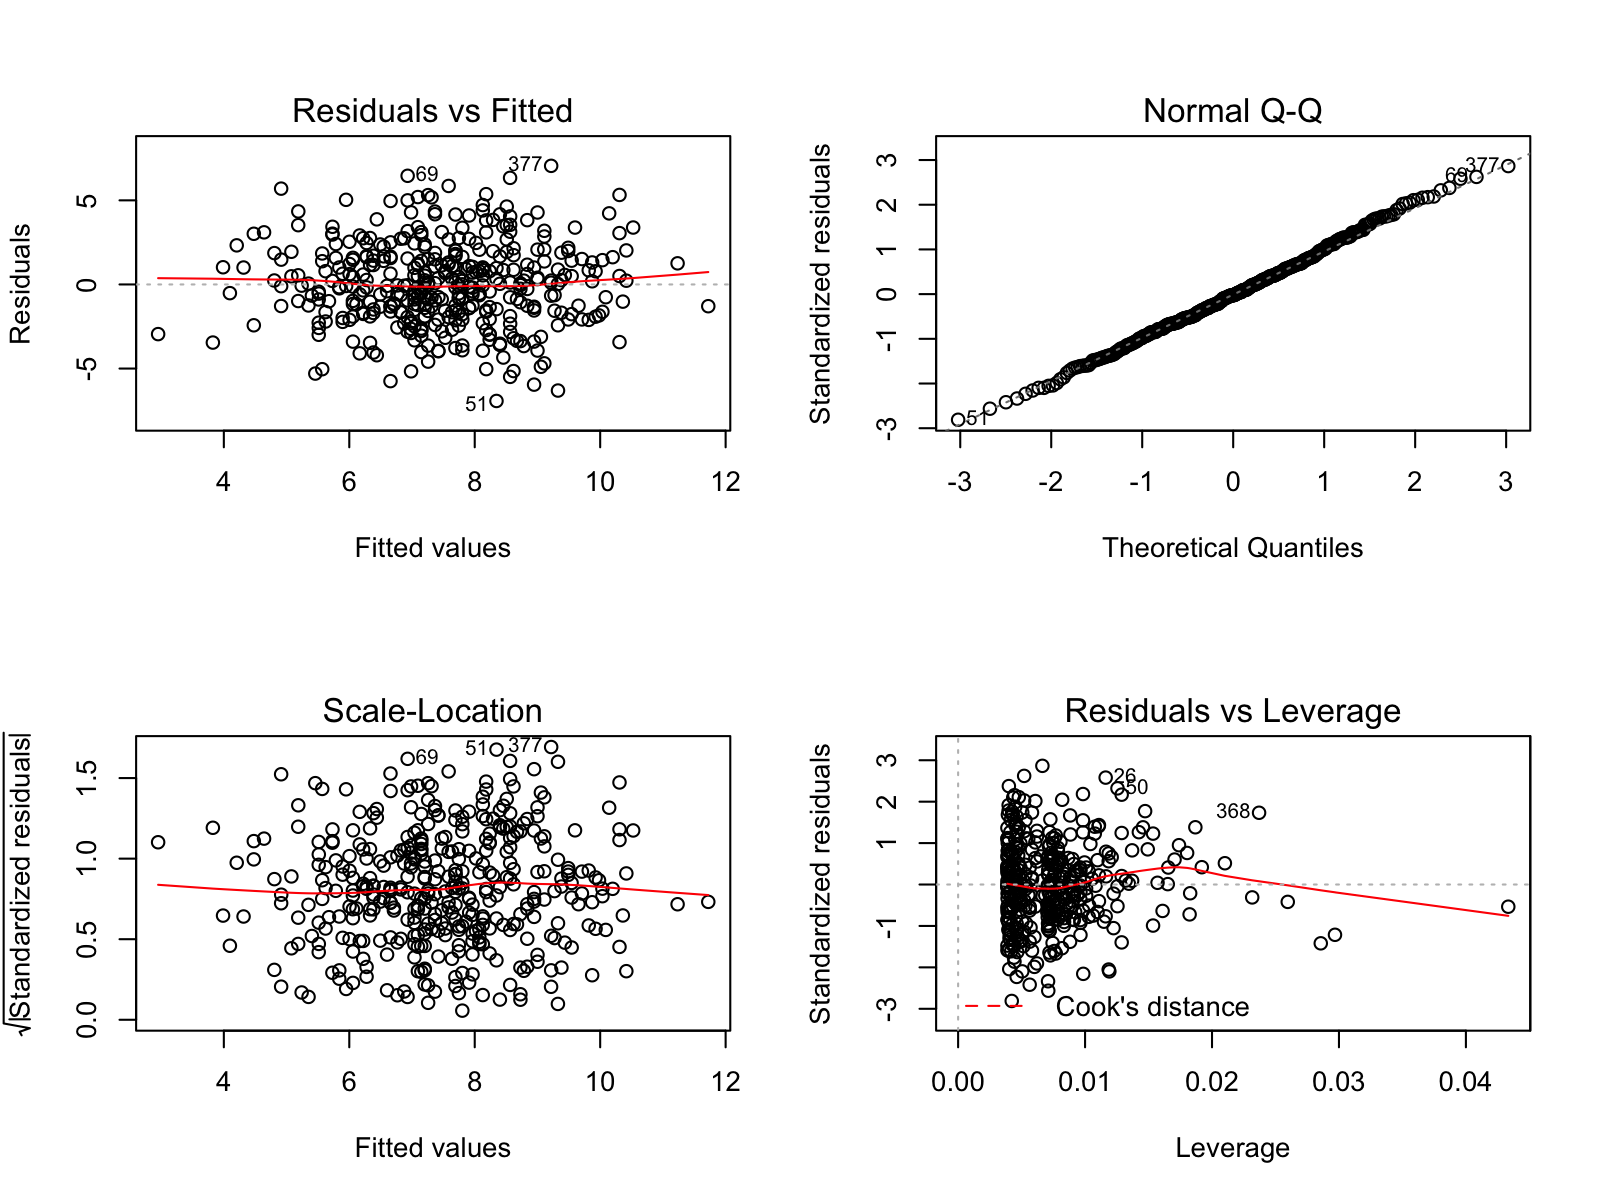
\includegraphics[width=0.8\textwidth]{MTH522_hw2_p2h.png}
	\end{center}
	\caption{.}
	\label{fig:MTH522_hw2_p2h}
\end{figure}

Residuals vs Leverage : Some outliers point out of [-2,2]. There are somee point that greatly exceeds (p+1)/n, then we can say that the corresponding point has high leverage (Page:99)

\newpage

\newpage
{\bf Problem 4} (Chapter 3 Exercises 15): This problem involves the Boston data set, which we saw in the lab for this chapter. We will now try to predict per capita crime rate using the other variables in this data set. In other words, per capita crime rate is the response, and the other variables are the predictors.

\item[(a)] For each predictor, fit a simple linear regression model to predict the response. Describe your results. In which of the models is there a statistically significant association between the predictor and the response? Create some plots to back up your assertions.



\begin{program}
	\begin{verbatim}
> library(MASS)
> attach(Boston)
> summary(Boston)

crim                zn             indus      
Min.   : 0.00632   Min.   :  0.00   Min.   : 0.46  
1st Qu.: 0.08204   1st Qu.:  0.00   1st Qu.: 5.19  
Median : 0.25651   Median :  0.00   Median : 9.69  
Mean   : 3.61352   Mean   : 11.36   Mean   :11.14  
3rd Qu.: 3.67708   3rd Qu.: 12.50   3rd Qu.:18.10  
Max.   :88.97620   Max.   :100.00   Max.   :27.74  
chas              nox               rm       
Min.   :0.00000   Min.   :0.3850   Min.   :3.561  
1st Qu.:0.00000   1st Qu.:0.4490   1st Qu.:5.886  
Median :0.00000   Median :0.5380   Median :6.208  
Mean   :0.06917   Mean   :0.5547   Mean   :6.285  
3rd Qu.:0.00000   3rd Qu.:0.6240   3rd Qu.:6.623  
Max.   :1.00000   Max.   :0.8710   Max.   :8.780  
age              dis              rad        
Min.   :  2.90   Min.   : 1.130   Min.   : 1.000  
1st Qu.: 45.02   1st Qu.: 2.100   1st Qu.: 4.000  
Median : 77.50   Median : 3.207   Median : 5.000  
Mean   : 68.57   Mean   : 3.795   Mean   : 9.549  
3rd Qu.: 94.08   3rd Qu.: 5.188   3rd Qu.:24.000  
Max.   :100.00   Max.   :12.127   Max.   :24.000  
tax           ptratio          black       
Min.   :187.0   Min.   :12.60   Min.   :  0.32  
1st Qu.:279.0   1st Qu.:17.40   1st Qu.:375.38  
Median :330.0   Median :19.05   Median :391.44  
Mean   :408.2   Mean   :18.46   Mean   :356.67  
3rd Qu.:666.0   3rd Qu.:20.20   3rd Qu.:396.23  
Max.   :711.0   Max.   :22.00   Max.   :396.90  
lstat            medv      
Min.   : 1.73   Min.   : 5.00  
1st Qu.: 6.95   1st Qu.:17.02  
Median :11.36   Median :21.20  
Mean   :12.65   Mean   :22.53  
3rd Qu.:16.95   3rd Qu.:25.00  
Max.   :37.97   Max.   :50.00  
	\end{verbatim}
\end{program}




\begin{program}
\begin{verbatim}
> fit.zn <- lm(crim ~ zn)
> summary(fit.zn)

Call:
lm(formula = crim ~ zn)

Residuals:
Min     1Q Median     3Q    Max 
-4.429 -4.222 -2.620  1.250 84.523 

Coefficients:
Estimate Std. Error t value Pr(>|t|)    
(Intercept)  4.45369    0.41722  10.675  < 2e-16 ***
zn          -0.07393    0.01609  -4.594 5.51e-06 ***
---
Signif. codes:  
0 ‘***’ 0.001 ‘**’ 0.01 ‘*’ 0.05 ‘.’ 0.1 ‘ ’ 1

Residual standard error: 8.435 on 504 degrees of freedom
Multiple R-squared:  0.04019,	Adjusted R-squared:  0.03828 
F-statistic:  21.1 on 1 and 504 DF,  p-value: 5.506e-06
\end{verbatim}
\end{program}

\begin{program}
\begin{verbatim}
> fit.indus <- lm(crim ~ indus)
> summary(fit.indus)

Call:
lm(formula = crim ~ indus)

Residuals:
Min      1Q  Median      3Q     Max 
-11.972  -2.698  -0.736   0.712  81.813 

Coefficients:
Estimate Std. Error t value Pr(>|t|)    
(Intercept) -2.06374    0.66723  -3.093  0.00209 ** 
indus        0.50978    0.05102   9.991  < 2e-16 ***
---
Signif. codes:  
0 ‘***’ 0.001 ‘**’ 0.01 ‘*’ 0.05 ‘.’ 0.1 ‘ ’ 1

Residual standard error: 7.866 on 504 degrees of freedom
Multiple R-squared:  0.1653,	Adjusted R-squared:  0.1637 
F-statistic: 99.82 on 1 and 504 DF,  p-value: < 2.2e-16
\end{verbatim}
\end{program}


\begin{program}
	\begin{verbatim}
> Boston$chas <- factor(chas, labels = c("N", "Y"))
> summary(Boston)
crim                zn             indus       chas         nox        
Min.   : 0.00632   Min.   :  0.00   Min.   : 0.46   N:471   Min.   :0.3850  
1st Qu.: 0.08204   1st Qu.:  0.00   1st Qu.: 5.19   Y: 35   1st Qu.:0.4490  
Median : 0.25651   Median :  0.00   Median : 9.69           Median :0.5380  
Mean   : 3.61352   Mean   : 11.36   Mean   :11.14           Mean   :0.5547  
3rd Qu.: 3.67708   3rd Qu.: 12.50   3rd Qu.:18.10           3rd Qu.:0.6240  
Max.   :88.97620   Max.   :100.00   Max.   :27.74           Max.   :0.8710  
rm             age              dis              rad              tax       
Min.   :3.561   Min.   :  2.90   Min.   : 1.130   Min.   : 1.000   Min.   :187.0  
1st Qu.:5.886   1st Qu.: 45.02   1st Qu.: 2.100   1st Qu.: 4.000   1st Qu.:279.0  
Median :6.208   Median : 77.50   Median : 3.207   Median : 5.000   Median :330.0  
Mean   :6.285   Mean   : 68.57   Mean   : 3.795   Mean   : 9.549   Mean   :408.2  
3rd Qu.:6.623   3rd Qu.: 94.08   3rd Qu.: 5.188   3rd Qu.:24.000   3rd Qu.:666.0  
Max.   :8.780   Max.   :100.00   Max.   :12.127   Max.   :24.000   Max.   :711.0  
ptratio          black            lstat            medv      
Min.   :12.60   Min.   :  0.32   Min.   : 1.73   Min.   : 5.00  
1st Qu.:17.40   1st Qu.:375.38   1st Qu.: 6.95   1st Qu.:17.02  
Median :19.05   Median :391.44   Median :11.36   Median :21.20  
Mean   :18.46   Mean   :356.67   Mean   :12.65   Mean   :22.53  
3rd Qu.:20.20   3rd Qu.:396.23   3rd Qu.:16.95   3rd Qu.:25.00  
Max.   :22.00   Max.   :396.90   Max.   :37.97   Max.   :50.00  
	
	
	> fit.chas <- lm(crim ~ chas)
	> summary(fit.chas)
	
	Call:
	lm(formula = crim ~ chas)
	
	Residuals:
	Min     1Q Median     3Q    Max 
	-3.738 -3.661 -3.435  0.018 85.232 
	
	Coefficients:
	Estimate Std. Error t value Pr(>|t|)    
	(Intercept)   3.7444     0.3961   9.453   <2e-16 ***
	chasY        -1.8928     1.5061  -1.257    0.209    
	---
	Signif. codes:  0 ‘***’ 0.001 ‘**’ 0.01 ‘*’ 0.05 ‘.’ 0.1 ‘ ’ 1
	
	Residual standard error: 8.597 on 504 degrees of freedom
	Multiple R-squared:  0.003124,	Adjusted R-squared:  0.001146 
	F-statistic: 1.579 on 1 and 504 DF,  p-value: 0.2094
	
	\end{verbatim}
\end{program}

\begin{program}
	\begin{verbatim}
	> fit.nox <- lm(crim ~ nox)
	> summary(fit.nox)
	
	Call:
	lm(formula = crim ~ nox)
	
	Residuals:
	Min      1Q  Median      3Q     Max 
	-12.371  -2.738  -0.974   0.559  81.728 
	
	Coefficients:
	Estimate Std. Error t value Pr(>|t|)    
	(Intercept)  -13.720      1.699  -8.073 5.08e-15 ***
	nox           31.249      2.999  10.419  < 2e-16 ***
	---
	Signif. codes:  0 ‘***’ 0.001 ‘**’ 0.01 ‘*’ 0.05 ‘.’ 0.1 ‘ ’ 1
	
	Residual standard error: 7.81 on 504 degrees of freedom
	Multiple R-squared:  0.1772,	Adjusted R-squared:  0.1756 
	F-statistic: 108.6 on 1 and 504 DF,  p-value: < 2.2e-16
	
	\end{verbatim}
\end{program}

\begin{program}
	\begin{verbatim}
	> fit.rm <- lm(crim ~ rm)
	> summary(fit.rm)
	
	Call:
	lm(formula = crim ~ rm)
	
	Residuals:
	Min     1Q Median     3Q    Max 
	-6.604 -3.952 -2.654  0.989 87.197 
	
	Coefficients:
	Estimate Std. Error t value Pr(>|t|)    
	(Intercept)   20.482      3.365   6.088 2.27e-09 ***
	rm            -2.684      0.532  -5.045 6.35e-07 ***
	---
	Signif. codes:  0 ‘***’ 0.001 ‘**’ 0.01 ‘*’ 0.05 ‘.’ 0.1 ‘ ’ 1
	
	Residual standard error: 8.401 on 504 degrees of freedom
	Multiple R-squared:  0.04807,	Adjusted R-squared:  0.04618 
	F-statistic: 25.45 on 1 and 504 DF,  p-value: 6.347e-07
	
	\end{verbatim}
\end{program}

\begin{program}
	\begin{verbatim}
	> fit.age <- lm(crim ~ age)
	> summary(fit.age)
	
	Call:
	lm(formula = crim ~ age)
	
	Residuals:
	Min     1Q Median     3Q    Max 
	-6.789 -4.257 -1.230  1.527 82.849 
	
	Coefficients:
	Estimate Std. Error t value Pr(>|t|)    
	(Intercept) -3.77791    0.94398  -4.002 7.22e-05 ***
	age          0.10779    0.01274   8.463 2.85e-16 ***
	---
	Signif. codes:  0 ‘***’ 0.001 ‘**’ 0.01 ‘*’ 0.05 ‘.’ 0.1 ‘ ’ 1
	
	Residual standard error: 8.057 on 504 degrees of freedom
	Multiple R-squared:  0.1244,	Adjusted R-squared:  0.1227 
	F-statistic: 71.62 on 1 and 504 DF,  p-value: 2.855e-16
	
	\end{verbatim}
\end{program}

\begin{program}
	\begin{verbatim}
	> fit.dis <- lm(crim ~ dis)
	> summary(fit.dis)
	
	Call:
	lm(formula = crim ~ dis)
	
	Residuals:
	Min     1Q Median     3Q    Max 
	-6.708 -4.134 -1.527  1.516 81.674 
	
	Coefficients:
	Estimate Std. Error t value Pr(>|t|)    
	(Intercept)   9.4993     0.7304  13.006   <2e-16 ***
	dis          -1.5509     0.1683  -9.213   <2e-16 ***
	---
	Signif. codes:  0 ‘***’ 0.001 ‘**’ 0.01 ‘*’ 0.05 ‘.’ 0.1 ‘ ’ 1
	
	Residual standard error: 7.965 on 504 degrees of freedom
	Multiple R-squared:  0.1441,	Adjusted R-squared:  0.1425 
	F-statistic: 84.89 on 1 and 504 DF,  p-value: < 2.2e-16
	
	\end{verbatim}
\end{program}

\begin{program}
	\begin{verbatim}
	> fit.rad <- lm(crim ~ rad)
	> summary(fit.rad)
	
	Call:
	lm(formula = crim ~ rad)
	
	Residuals:
	Min      1Q  Median      3Q     Max 
	-10.164  -1.381  -0.141   0.660  76.433 
	
	Coefficients:
	Estimate Std. Error t value Pr(>|t|)    
	(Intercept) -2.28716    0.44348  -5.157 3.61e-07 ***
	rad          0.61791    0.03433  17.998  < 2e-16 ***
	---
	Signif. codes:  0 ‘***’ 0.001 ‘**’ 0.01 ‘*’ 0.05 ‘.’ 0.1 ‘ ’ 1
	
	Residual standard error: 6.718 on 504 degrees of freedom
	Multiple R-squared:  0.3913,	Adjusted R-squared:   0.39 
	F-statistic: 323.9 on 1 and 504 DF,  p-value: < 2.2e-16
	
	\end{verbatim}
\end{program}

\begin{program}
	\begin{verbatim}
	> fit.tax <- lm(crim ~ tax)
	> summary(fit.tax)
	
	Call:
	lm(formula = crim ~ tax)
	
	Residuals:
	Min      1Q  Median      3Q     Max 
	-12.513  -2.738  -0.194   1.065  77.696 
	
	Coefficients:
	Estimate Std. Error t value Pr(>|t|)    
	(Intercept) -8.528369   0.815809  -10.45   <2e-16 ***
	tax          0.029742   0.001847   16.10   <2e-16 ***
	---
	Signif. codes:  0 ‘***’ 0.001 ‘**’ 0.01 ‘*’ 0.05 ‘.’ 0.1 ‘ ’ 1
	
	Residual standard error: 6.997 on 504 degrees of freedom
	Multiple R-squared:  0.3396,	Adjusted R-squared:  0.3383 
	F-statistic: 259.2 on 1 and 504 DF,  p-value: < 2.2e-16
	
	\end{verbatim}
\end{program}



\begin{program}
	\begin{verbatim}
	> fit.ptratio <- lm(crim ~ ptratio)
	> summary(fit.ptratio)
	
	Call:
	lm(formula = crim ~ ptratio)
	
	Residuals:
	Min     1Q Median     3Q    Max 
	-7.654 -3.985 -1.912  1.825 83.353 
	
	Coefficients:
	Estimate Std. Error t value Pr(>|t|)    
	(Intercept) -17.6469     3.1473  -5.607 3.40e-08 ***
	ptratio       1.1520     0.1694   6.801 2.94e-11 ***
	---
	Signif. codes:  0 ‘***’ 0.001 ‘**’ 0.01 ‘*’ 0.05 ‘.’ 0.1 ‘ ’ 1
	
	Residual standard error: 8.24 on 504 degrees of freedom
	Multiple R-squared:  0.08407,	Adjusted R-squared:  0.08225 
	F-statistic: 46.26 on 1 and 504 DF,  p-value: 2.943e-11
	
	\end{verbatim}
\end{program}


\begin{program}
	\begin{verbatim}
	> fit.black <- lm(crim ~ black)
	> summary(fit.black)
	
	Call:
	lm(formula = crim ~ black)
	
	Residuals:
	Min      1Q  Median      3Q     Max 
	-13.756  -2.299  -2.095  -1.296  86.822 
	
	Coefficients:
	Estimate Std. Error t value Pr(>|t|)    
	(Intercept) 16.553529   1.425903  11.609   <2e-16 ***
	black       -0.036280   0.003873  -9.367   <2e-16 ***
	---
	Signif. codes:  0 ‘***’ 0.001 ‘**’ 0.01 ‘*’ 0.05 ‘.’ 0.1 ‘ ’ 1
	
	Residual standard error: 7.946 on 504 degrees of freedom
	Multiple R-squared:  0.1483,	Adjusted R-squared:  0.1466 
	F-statistic: 87.74 on 1 and 504 DF,  p-value: < 2.2e-16
	
	\end{verbatim}
\end{program}


\begin{program}
	\begin{verbatim}
	> fit.lstat <- lm(crim ~ lstat)
	> summary(fit.lstat)
	
	Call:
	lm(formula = crim ~ lstat)
	
	Residuals:
	Min      1Q  Median      3Q     Max 
	-13.925  -2.822  -0.664   1.079  82.862 
	
	Coefficients:
	Estimate Std. Error t value Pr(>|t|)    
	(Intercept) -3.33054    0.69376  -4.801 2.09e-06 ***
	lstat        0.54880    0.04776  11.491  < 2e-16 ***
	---
	Signif. codes:  0 ‘***’ 0.001 ‘**’ 0.01 ‘*’ 0.05 ‘.’ 0.1 ‘ ’ 1
	
	Residual standard error: 7.664 on 504 degrees of freedom
	Multiple R-squared:  0.2076,	Adjusted R-squared:  0.206 
	F-statistic:   132 on 1 and 504 DF,  p-value: < 2.2e-16
	
	\end{verbatim}
\end{program}


\begin{program}
	\begin{verbatim}
	> fit.medv <- lm(crim ~ medv)
	> summary(fit.medv)
	
	Call:
	lm(formula = crim ~ medv)
	
	Residuals:
	Min     1Q Median     3Q    Max 
	-9.071 -4.022 -2.343  1.298 80.957 
	
	Coefficients:
	Estimate Std. Error t value Pr(>|t|)    
	(Intercept) 11.79654    0.93419   12.63   <2e-16 ***
	medv        -0.36316    0.03839   -9.46   <2e-16 ***
	---
	Signif. codes:  0 ‘***’ 0.001 ‘**’ 0.01 ‘*’ 0.05 ‘.’ 0.1 ‘ ’ 1
	
	Residual standard error: 7.934 on 504 degrees of freedom
	Multiple R-squared:  0.1508,	Adjusted R-squared:  0.1491 
	F-statistic: 89.49 on 1 and 504 DF,  p-value: < 2.2e-16
	
	\end{verbatim}
\end{program}


\newpage
....
\newpage
....
\newpage
....
\newpage
....
\newpage
....
\newpage
....
\newpage

For each predictor, we fit a simple linear regression model. 
For significant predictors, we have to test $H_0 : B_1 = 0$ and for necessary p-values we can reject this null hypothesis.
\\The "chas"  predictor has the largest p-value  and other all predictors have a very small p-values, so we can say that  except "chas" predictor, there is a statistically significant association between the predictor and the response


\newpage

\item[(b)] Fit a multiple regression model to predict the response using all of the predictors. Describe your results. For which predictors can we reject the null hypothesis H0 : βj = 0?


\begin{program}
	\begin{verbatim}
	> fit.all <- lm(crim ~ ., data = Boston)
	> summary(fit.all)
	
	Call:
	lm(formula = crim ~ ., data = Boston)
	
	Residuals:
	Min     1Q Median     3Q    Max 
	-9.924 -2.120 -0.353  1.019 75.051 
	
	Coefficients:
	              Estimate Std. Error t value Pr(>|t|)    
	(Intercept)  17.033228   7.234903   2.354 0.018949 *  
	zn            0.044855   0.018734   2.394 0.017025 *  
	indus        -0.063855   0.083407  -0.766 0.444294    
	chasY        -0.749134   1.180147  -0.635 0.525867    
	nox         -10.313535   5.275536  -1.955 0.051152 .  
	rm            0.430131   0.612830   0.702 0.483089    
	age           0.001452   0.017925   0.081 0.935488    
	dis          -0.987176   0.281817  -3.503 0.000502 ***
	rad           0.588209   0.088049   6.680 6.46e-11 ***
	tax          -0.003780   0.005156  -0.733 0.463793    
	ptratio      -0.271081   0.186450  -1.454 0.146611    
	black        -0.007538   0.003673  -2.052 0.040702 *  
	lstat         0.126211   0.075725   1.667 0.096208 .  
	medv         -0.198887   0.060516  -3.287 0.001087 ** 
	---
	Signif. codes:  0 ‘***’ 0.001 ‘**’ 0.01 ‘*’ 0.05 ‘.’ 0.1 ‘ ’ 1
	
	Residual standard error: 6.439 on 492 degrees of freedom
	Multiple R-squared:  0.454,	Adjusted R-squared:  0.4396 
	F-statistic: 31.47 on 13 and 492 DF,  p-value: < 2.2e-16
	
	\end{verbatim}
\end{program}

\begin{lstlisting}
Following predictor has small p-values and we may reject the null hypothesis
	zn          0.017025
	dis         0.000502
	rad         6.46e-11
	black       0.040702  
	medv        0.001087 
\end{lstlisting}




\item[(c)] How do your results from (a) compare to your results from (b)? Create a plot displaying the univariate regression coefficients from (a) on the x-axis, and the multiple regression coefficients from (b) on the y-axis. That is, each predictor is displayed as a single point in the plot. Its coefficient in a simple linear regres- sion model is shown on the x-axis, and its coefficient estimate in the multiple linear regression model is shown on the y-axis.

\begin{program}
	\begin{verbatim}
	> fit.uni.x = c(coefficients(fit.zn)[2],
	>+       coefficients(fit.indus)[2],
	> +       coefficients(fit.chas)[2],
	> +       coefficients(fit.nox)[2],
	> +       coefficients(fit.rm)[2],
	> +       coefficients(fit.age)[2],
	> +       coefficients(fit.dis)[2],
	> +       coefficients(fit.rad)[2],
	> +       coefficients(fit.tax)[2],
	> +       coefficients(fit.ptratio)[2],
	> +       coefficients(fit.black)[2],
	> +       coefficients(fit.lstat)[2],
	> +       coefficients(fit.medv)[2])
	> fit.mul.y = coefficients(fit.all)[2:14]
	> plot(fit.uni.x, fit.mul.y)
	
	> dev.copy(png,"MTH522_hw2_p3c.png",width=8,height=6,units="in",res=200)
	> dev.off()	
	\end{verbatim}
	\caption{The R code used to generate Figure.\ \ref{fig:MTH522_hw2_p3c}.}
\end{program}


\begin{figure}[htb]
	\begin{center}
		
\includegraphics[width=0.8\textwidth]{MTH522_hw2_p3c.png}
	\end{center}
	\caption{.}
	\label{fig:MTH522_hw2_p3c}
\end{figure}


\begin{program}
	\begin{verbatim}

lets find out which univariate regression coefficients is <-10

	> print(fit.uni.x)
	
	         zn       indus       chasY         nox          rm         age 
	-0.07393498  0.50977633 -1.89277655 31.24853120 -2.68405122  0.10778623 
	        dis         rad         tax     ptratio       black       lstat 
	-1.55090168  0.61791093  0.02974225  1.15198279 -0.03627964  0.54880478 
	medv 
	-0.36315992 

Univariate regression coefficients for nox is  approximately 31 and from 
Figure 8 multiple regression coefficients is approximately -10
	\end{verbatim}
\end{program}

\newpage
...
\newpage





\item[(d)] Is there evidence of non-linear association between any of the predictors and the response? To answer this question, for each predictor X, fit a model of the form
$Y = B_0 +B_1X +B_2X^2 +B_3X^3 +E $




\begin{program}
	\begin{verbatim}
	> library(MASS)
	> attach(Boston)
	> fit.zn <- lm(crim ~ poly(zn, 3))
	> summary(fit.zn)
	
	Call:
	lm(formula = crim ~ poly(zn, 3))
	
	Residuals:
	Min     1Q Median     3Q    Max 
	-4.821 -4.614 -1.294  0.473 84.130 
	
	Coefficients:
	             Estimate Std. Error t value Pr(>|t|)    
	(Intercept)    3.6135     0.3722   9.709  < 2e-16 ***
	poly(zn, 3)1 -38.7498     8.3722  -4.628  4.7e-06 ***
	poly(zn, 3)2  23.9398     8.3722   2.859  0.00442 ** 
	poly(zn, 3)3 -10.0719     8.3722  -1.203  0.22954    
	---
	Signif. codes:  0 ‘***’ 0.001 ‘**’ 0.01 ‘*’ 0.05 ‘.’ 0.1 ‘ ’ 1
	
	Residual standard error: 8.372 on 502 degrees of freedom
	Multiple R-squared:  0.05824,	Adjusted R-squared:  0.05261 
	F-statistic: 10.35 on 3 and 502 DF,  p-value: 1.281e-06
	
	\end{verbatim}
\end{program}


\begin{program}
	\begin{verbatim}
	> fit.indus <- lm(crim ~ poly(indus, 3))
	> summary(fit.indus)
	
	Call:
	lm(formula = crim ~ poly(indus, 3))
	
	Residuals:
	Min     1Q Median     3Q    Max 
	-8.278 -2.514  0.054  0.764 79.713 
	
	Coefficients:
	             Estimate Std. Error t value Pr(>|t|)    
	(Intercept)        3.614      0.330  10.950  < 2e-16 ***
	poly(indus, 3)1   78.591      7.423  10.587  < 2e-16 ***
	poly(indus, 3)2  -24.395      7.423  -3.286  0.00109 ** 
	poly(indus, 3)3  -54.130      7.423  -7.292  1.2e-12 ***
	---
	Signif. codes:  0 ‘***’ 0.001 ‘**’ 0.01 ‘*’ 0.05 ‘.’ 0.1 ‘ ’ 1
	
	Residual standard error: 7.423 on 502 degrees of freedom
	Multiple R-squared:  0.2597,	Adjusted R-squared:  0.2552 
	F-statistic: 58.69 on 3 and 502 DF,  p-value: < 2.2e-16
	
	\end{verbatim}
\end{program}


\begin{program}
	\begin{verbatim}
	> fit.nox <- lm(crim ~ poly(nox, 3))
	> summary(fit.nox)
	
	Call:
	lm(formula = crim ~ poly(nox, 3))
	
	Residuals:
	Min     1Q Median     3Q    Max 
	-9.110 -2.068 -0.255  0.739 78.302 
	
	Coefficients:
	              Estimate Std. Error t value Pr(>|t|)    
	(Intercept)     3.6135     0.3216  11.237  < 2e-16 ***
	poly(nox, 3)1  81.3720     7.2336  11.249  < 2e-16 ***
	poly(nox, 3)2 -28.8286     7.2336  -3.985 7.74e-05 ***
	poly(nox, 3)3 -60.3619     7.2336  -8.345 6.96e-16 ***
	---
	Signif. codes:  0 ‘***’ 0.001 ‘**’ 0.01 ‘*’ 0.05 ‘.’ 0.1 ‘ ’ 1
	
	Residual standard error: 7.234 on 502 degrees of freedom
	Multiple R-squared:  0.297,	Adjusted R-squared:  0.2928 
	F-statistic: 70.69 on 3 and 502 DF,  p-value: < 2.2e-16
	\end{verbatim}
\end{program}


\begin{program}
	\begin{verbatim}
	> fit.rm <- lm(crim ~ poly(rm, 3))
	> summary(fit.rm)
	
	Call:
	lm(formula = crim ~ poly(rm, 3))
	
	Residuals:
	Min      1Q  Median      3Q     Max 
	-18.485  -3.468  -2.221  -0.015  87.219 
	
	Coefficients:
	             Estimate Std. Error t value Pr(>|t|)    
	(Intercept)    3.6135     0.3703   9.758  < 2e-16 ***
	poly(rm, 3)1 -42.3794     8.3297  -5.088 5.13e-07 ***
	poly(rm, 3)2  26.5768     8.3297   3.191  0.00151 ** 
	poly(rm, 3)3  -5.5103     8.3297  -0.662  0.50858    
	---
	Signif. codes:  0 ‘***’ 0.001 ‘**’ 0.01 ‘*’ 0.05 ‘.’ 0.1 ‘ ’ 1
	
	Residual standard error: 8.33 on 502 degrees of freedom
	Multiple R-squared:  0.06779,	Adjusted R-squared:  0.06222 
	F-statistic: 12.17 on 3 and 502 DF,  p-value: 1.067e-07
	
	\end{verbatim}
\end{program}


\begin{program}
	\begin{verbatim}
	> fit.age <- lm(crim ~ poly(age, 3))
	> summary(fit.age)
	
	Call:
	lm(formula = crim ~ poly(age, 3))
	
	Residuals:
	Min     1Q Median     3Q    Max 
	-9.762 -2.673 -0.516  0.019 82.842 
	
	Coefficients:
	Estimate Std. Error t value Pr(>|t|)    
	(Intercept)     3.6135     0.3485  10.368  < 2e-16 ***
	poly(age, 3)1  68.1820     7.8397   8.697  < 2e-16 ***
	poly(age, 3)2  37.4845     7.8397   4.781 2.29e-06 ***
	poly(age, 3)3  21.3532     7.8397   2.724  0.00668 ** 
	---
	Signif. codes:  0 ‘***’ 0.001 ‘**’ 0.01 ‘*’ 0.05 ‘.’ 0.1 ‘ ’ 1
	
	Residual standard error: 7.84 on 502 degrees of freedom
	Multiple R-squared:  0.1742,	Adjusted R-squared:  0.1693 
	F-statistic: 35.31 on 3 and 502 DF,  p-value: < 2.2e-16
	
	\end{verbatim}
\end{program}


\begin{program}
	\begin{verbatim}
	> fit.dis <- lm(crim ~ poly(dis, 3))
	> summary(fit.dis)
	
	Call:
	lm(formula = crim ~ poly(dis, 3))
	
	Residuals:
	Min      1Q  Median      3Q     Max 
	-10.757  -2.588   0.031   1.267  76.378 
	
	Coefficients:
	             Estimate Std. Error t value Pr(>|t|)    
	(Intercept)     3.6135     0.3259  11.087  < 2e-16 ***
	poly(dis, 3)1 -73.3886     7.3315 -10.010  < 2e-16 ***
	poly(dis, 3)2  56.3730     7.3315   7.689 7.87e-14 ***
	poly(dis, 3)3 -42.6219     7.3315  -5.814 1.09e-08 ***
	---
	Signif. codes:  0 ‘***’ 0.001 ‘**’ 0.01 ‘*’ 0.05 ‘.’ 0.1 ‘ ’ 1
	
	Residual standard error: 7.331 on 502 degrees of freedom
	Multiple R-squared:  0.2778,	Adjusted R-squared:  0.2735 
	F-statistic: 64.37 on 3 and 502 DF,  p-value: < 2.2e-16
	\end{verbatim}
\end{program}


\begin{program}
	\begin{verbatim}
	> fit.rad <- lm(crim ~ poly(rad, 3))
	> summary(fit.rad)
	
	Call:
	lm(formula = crim ~ poly(rad, 3))
	
	Residuals:
	Min      1Q  Median      3Q     Max 
	-10.381  -0.412  -0.269   0.179  76.217 
	
	Coefficients:
	             Estimate Std. Error t value Pr(>|t|)    
	(Intercept)     3.6135     0.2971  12.164  < 2e-16 ***
	poly(rad, 3)1 120.9074     6.6824  18.093  < 2e-16 ***
	poly(rad, 3)2  17.4923     6.6824   2.618  0.00912 ** 
	poly(rad, 3)3   4.6985     6.6824   0.703  0.48231    
	---
	Signif. codes:  0 ‘***’ 0.001 ‘**’ 0.01 ‘*’ 0.05 ‘.’ 0.1 ‘ ’ 1
	
	Residual standard error: 6.682 on 502 degrees of freedom
	Multiple R-squared:    0.4,	Adjusted R-squared:  0.3965 
	F-statistic: 111.6 on 3 and 502 DF,  p-value: < 2.2e-16
	\end{verbatim}
\end{program}


\begin{program}
	\begin{verbatim}
	> fit.tax <- lm(crim ~ poly(tax, 3))
	> summary(fit.tax)
	
	Call:
	lm(formula = crim ~ poly(tax, 3))
	
	Residuals:
	Min      1Q  Median      3Q     Max 
	-13.273  -1.389   0.046   0.536  76.950 
	
	Coefficients:
	             Estimate Std. Error t value Pr(>|t|)    
	(Intercept)     3.6135     0.3047  11.860  < 2e-16 ***
	poly(tax, 3)1 112.6458     6.8537  16.436  < 2e-16 ***
	poly(tax, 3)2  32.0873     6.8537   4.682 3.67e-06 ***
	poly(tax, 3)3  -7.9968     6.8537  -1.167    0.244    
	---
	Signif. codes:  0 ‘***’ 0.001 ‘**’ 0.01 ‘*’ 0.05 ‘.’ 0.1 ‘ ’ 1
	
	Residual standard error: 6.854 on 502 degrees of freedom
	Multiple R-squared:  0.3689,	Adjusted R-squared:  0.3651 
	F-statistic:  97.8 on 3 and 502 DF,  p-value: < 2.2e-16
	
	\end{verbatim}
\end{program}


\begin{program}
	\begin{verbatim}
	> fit.ptratio <- lm(crim ~ poly(ptratio, 3))
	> summary(fit.ptratio)
	
	Call:
	lm(formula = crim ~ poly(ptratio, 3))
	
	Residuals:
	Min     1Q Median     3Q    Max 
	-6.833 -4.146 -1.655  1.408 82.697 
	
	Coefficients:
	              Estimate Std. Error t value Pr(>|t|)    
	(Intercept)          3.614      0.361  10.008  < 2e-16 ***
	poly(ptratio, 3)1   56.045      8.122   6.901 1.57e-11 ***
	poly(ptratio, 3)2   24.775      8.122   3.050  0.00241 ** 
	poly(ptratio, 3)3  -22.280      8.122  -2.743  0.00630 ** 
	---
	Signif. codes:  0 ‘***’ 0.001 ‘**’ 0.01 ‘*’ 0.05 ‘.’ 0.1 ‘ ’ 1
	
	Residual standard error: 8.122 on 502 degrees of freedom
	Multiple R-squared:  0.1138,	Adjusted R-squared:  0.1085 
	F-statistic: 21.48 on 3 and 502 DF,  p-value: 4.171e-13
	
	\end{verbatim}
\end{program}


\begin{program}
	\begin{verbatim}
	> fit.black <- lm(crim ~ poly(black, 3))
	> summary(fit.black)
	
	Call:
	lm(formula = crim ~ poly(black, 3))
	
	Residuals:
	Min      1Q  Median      3Q     Max 
	-13.096  -2.343  -2.128  -1.439  86.790 
	
	Coefficients:
	             Estimate Std. Error t value Pr(>|t|)    
	(Intercept)       3.6135     0.3536  10.218   <2e-16 ***
	poly(black, 3)1 -74.4312     7.9546  -9.357   <2e-16 ***
	poly(black, 3)2   5.9264     7.9546   0.745    0.457    
	poly(black, 3)3  -4.8346     7.9546  -0.608    0.544    
	---
	Signif. codes:  0 ‘***’ 0.001 ‘**’ 0.01 ‘*’ 0.05 ‘.’ 0.1 ‘ ’ 1
	
	Residual standard error: 7.955 on 502 degrees of freedom
	Multiple R-squared:  0.1498,	Adjusted R-squared:  0.1448 
	F-statistic: 29.49 on 3 and 502 DF,  p-value: < 2.2e-16
	
	\end{verbatim}
\end{program}


\begin{program}
	\begin{verbatim}
	> fit.lstat <- lm(crim ~ poly(lstat, 3))
	> summary(fit.lstat)
	
	Call:
	lm(formula = crim ~ poly(lstat, 3))
	
	Residuals:
	Min      1Q  Median      3Q     Max 
	-15.234  -2.151  -0.486   0.066  83.353 
	
	Coefficients:
	              Estimate Std. Error t value Pr(>|t|)    
	(Intercept)       3.6135     0.3392  10.654   <2e-16 ***
	poly(lstat, 3)1  88.0697     7.6294  11.543   <2e-16 ***
	poly(lstat, 3)2  15.8882     7.6294   2.082   0.0378 *  
	poly(lstat, 3)3 -11.5740     7.6294  -1.517   0.1299    
	---
	Signif. codes:  0 ‘***’ 0.001 ‘**’ 0.01 ‘*’ 0.05 ‘.’ 0.1 ‘ ’ 1
	
	Residual standard error: 7.629 on 502 degrees of freedom
	Multiple R-squared:  0.2179,	Adjusted R-squared:  0.2133 
	F-statistic: 46.63 on 3 and 502 DF,  p-value: < 2.2e-16
	\end{verbatim}
\end{program}


\begin{program}
	\begin{verbatim}
	> fit.medv <- lm(crim ~ poly(medv, 3))
	> summary(fit.medv)
	
	Call:
	lm(formula = crim ~ poly(medv, 3))
	
	Residuals:
	Min      1Q  Median      3Q     Max 
	-24.427  -1.976  -0.437   0.439  73.655 
	
	Coefficients:
	              Estimate Std. Error t value Pr(>|t|)    
	(Intercept)       3.614      0.292  12.374  < 2e-16 ***
	poly(medv, 3)1  -75.058      6.569 -11.426  < 2e-16 ***
	poly(medv, 3)2   88.086      6.569  13.409  < 2e-16 ***
	poly(medv, 3)3  -48.033      6.569  -7.312 1.05e-12 ***
	---
	Signif. codes:  0 ‘***’ 0.001 ‘**’ 0.01 ‘*’ 0.05 ‘.’ 0.1 ‘ ’ 1
	
	Residual standard error: 6.569 on 502 degrees of freedom
	Multiple R-squared:  0.4202,	Adjusted R-squared:  0.4167 
	F-statistic: 121.3 on 3 and 502 DF,  p-value: < 2.2e-16	
	\end{verbatim}
\end{program}


\newpage
...
\newpage
 ...
 \newpage
 ...
 \newpage
 ...
 \newpage
 ...
 \newpage
 
 As predictor : zn - rm - rad - tax - lstat - the p-values for  poly()3 coefficient is to large and it is not  statistically significant.
 As predictor : black- the p-values for  poly()2 and poly()3 coefficient is to large and it is not statistically significant.
 As predictor : indus - nox - age - dis - ptratio - medv - the p-values suggest of the cubic fit.
No non-linear association between any of the predictors and the response  is visible.
\newpage




\end{itemize}
\end{document}



